\documentclass[12pt]{report}
\usepackage{cs_thesis}
\usepackage[pdftex]{graphicx}
\usepackage[utf8]{inputenc}
\usepackage{amsmath}

\title{THE ICUB HUMANOID ROBOT \\ PROPOSAL}
\author{Semih Onay}

\program{Computer Science}

\supervisor{Assistant Professor Elena Battini Sönmez}


\begin{document}

\makecstitle

\chapter*{ABSTRACT}
The iCub is a humanoid robot developed at Istituto Italiano di Tecnologia (IIT) as part of the European Union project; RobotCub and later adopted by more than 20 laboratories around the world. Research team have developed a computer simulator to experiment new techniques without having a physical robot.\cite{iCub}

\chapter{INTRODUCTION}
\pagenumbering{arabic}
The iCub simulator is designed to be as accurate as real world psychics and dynamics. Construction based on directly from first prototype simulation environment Webots\cite{webots}. Webots is expensive and had limited access to source code which made hard to modify source code in order to add some properties. Then iCub simulation created. Simulation environment uses ODE(Open Dynamics Engine)\cite{ode} to simulate body movement and collision detection algorithms to measure psychical interaction with the world.ODE is used in wide range of projects like Gazebo project.\cite{gazebo}ODE is an open source physics engine for authoring tools, computer games,etc. It uses OpenGL renderer and it has some disadvantages due to limitation of OpenGL engine computation efficiency on complex structures.iCub simulation uses OpenGL directly via SDL which helps to render complex robot movements and computation efficient simulation observations.\cite{sdl} Simulator is free and available to anyone who interested in robotics and learning about basics of robotics.\newpage

\chapter{PROBLEM STATEMENT}

There are many different grounded approaches for modelling language, in which linguistic abilities are developed through the direct interaction between the cognitive agents and the physical world have been proposed. In these models, the external world plays an essential role in shaping the language used by these cognitive systems. Language is therefore grounded in the cognitive and sensorimotor knowledge of the agents.\cite{cag} The grounding of language in autonomous cognitive robots requires a direct grounding of the agent’s basic wordbook. This assumes the ability to link perceptual and internal representations to symbols. In this modeling paradigm, artificial agents are asked to associate features of objects to words, where this association is self- organized by the agents itself. An agent discovers autonomously certain features that are peculiar to a given object and learns from a model, which is usually another agent, to associate the feature to an arbitrary word.
\chapter{LITERATURE SURVEY}

Development of simulator is described by abstraction of parts to handle complex instructions more precisely and efficient. Some other external software libraries are used to reduce required time to animate given parts of robots body from parameters. Abstractions made it easy to implement new methods,algorithms into a simulation environment. Understanding of these libraries are the key of creating new interfaces and methods to robot in virtual world.
Action primitives are pre-defined inside a simulation environment to extend capability of creating new interfaces to virtual simulation world and can be changed or taught as different languages which helps to extend knowledge about languages.\cite{angelo}

Using artificial brain system utilizes recurrent loops to help the system understand new things having a grammatical structure, and it is even capable of linking two sentences together or predicting the end of a sentence before it is provided. This could be important as this system could be used to help understand the way the human brain processes language.\cite{xavier}

When concepts become more uninvolved from the physical objects and more linked with ‘mental events’, they become hugely abstract. Furthermore, to testify the complexity of the problem. It has been proposed to classify terms that refer to emotions in a distinct group from concrete and abstract words. Given the current debate in the field and the complexity of the matter, nowadays the task of creating higher-order concepts through language has been proved an extremely complex task on cognitive robotics.\cite{venuto}
\newpage


\chapter{METHODOLOGY}

Research will go on a computer simulation model of the iCub robot. The simulator allows to create realistic scenarios in where robot can interact with a virtual world and physical limitations and interactions that occur between the virtual world is simulated using open source library which is ODE (Open Dynamics Engine) to provide accurate simulation of body dynamics. 
\begin{figure}[!h]
\begin{center}
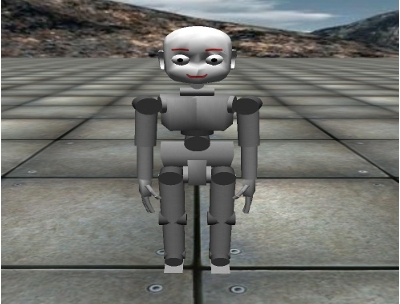
\includegraphics[scale=1.3]{iCubSim.jpg}
\caption{iCub on simulation}
\end{center}
\end{figure}
The iCub simulation was developed on the top of YARP(Yet Another Robot Platform)\cite{yarp}.YARP is a set of open source libraries that supports modularity by using abstraction method in softwares to handle common difficulties in robotics area which are know as modularity algorithms and hardware interfaces and OS platforms.To deal with OS spesific builds,requires to use cross-platform build tools such as CMake\cite{cmake} and ACE\cite{ace}.

YARP is providing platform independence. First abstraction can be described as a protocols.Main YARP protocol manages inter-process communications in operating systems. It can deliver process messages of any size across the network by using different protocols.
\newpage
Second abstraction is about hardware communications.The method is to define interface for class of devices to fold native coded APIs.Changes in hardwares requires changes in API calls via linking suitable libraries to encapsulate hardware dependency problems. 
These two abstraction combined to use remote device drives where that can be accessed across the network like a parallel processing.

\begin{figure}[!h]
\begin{center}
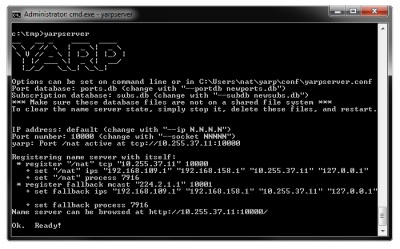
\includegraphics[scale=1.0]{yarpServer.jpg}
\caption{yarpServer running on Windows x86}
\end{center}
\end{figure}

\begin{figure}[!h]
\begin{center}
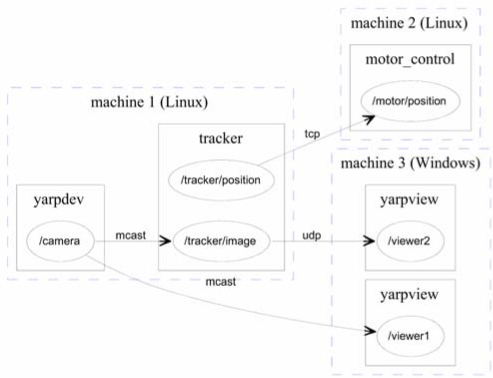
\includegraphics[scale=0.4]{network.jpg}
\caption{YARP Work Flow}
\end{center}
\end{figure}
The purpose of YARP ports are to move data from threads to threads over the processes. Flow of the data can be configured and observed from command-line at real-time.Port can receive or send data from any other port.Connections between ports can be modified easily with using different protocols such as TCP(Transmission Control Protocol) and UDP(User Datagram Protocol). The choice of protocol is depends on quality of message transmission or response time.Using TCP is for reliability and UDP is for speed with effect on unreliable transmissions.
\newpage

\chapter{CONCLUSION}
The latest stable version of the iCub Simulator will be used to implement some action primitives into a default library to extend it's knowledge about different languages such as Turkish language. Compiling the source code of YARP and iCub Simulator may difficult due to platform dependent system environment variables. Many unix systems has some advantages about solving dependency problems via package managers.

\begin{thebibliography}{9}
\bibitem{iCub}iCub : \underline{http://icub.org}
\bibitem{webots}Webots : \underline{http://cyberbotics.com}
\bibitem{ode}ODE(Open Dynamics Engine) : \underline{http://opende.sourceforge.net}
\bibitem{gazebo}GAZEBO : \underline{http://gazebosim.org}
\bibitem{angelo}The iCub humanoid robot:
an open platform for research in embodied cognition , Giorgio Metta, Giulio Sandini, David Vernon, Lorenzo Natale, Francesco Nori
\bibitem{cag}Cangelosi \& Steels, Evolving grounded communication for robots. Trends in Cognitive Sciences
\bibitem{venuto}Imagery, context availability,
contextual constraint, and abstractness. In Proceedings of the 23rd Annual Conference of the Cognitive Science Society Barsalou, Paivio, Yuille, \& Madigan ; Wiemer-Hastings
\bibitem{xavier}Real-Time Parallel Processing of Grammatical Structure in the Fronto-Striatal System: A Recurrent Network Simulation Study Using Reservoir Computing , Xavier Hinaut, Peter Ford Dominey
\bibitem{sdl}SDL : \underline{http://libsdl.org}
\bibitem{yarp}YARP : \underline{http://wiki.icub.org/yarpdoc/index.html}
\bibitem{cmake}CMake : \underline{http://cmake.org} 
\bibitem{ace}Adaptive Communication Environment : \underline{http://dre.vanderbilt.edu/$\sim$schmidt/ACE.html}
\bibitem{resource}The iCub humanoid robot:an open platform for research in embodied cognition,Giorgio Metta,Giulio Sandini,David Vernon,Lorenzo Natale,Francesco Nori
\bibitem{resource,resource2}The iCub Humanoid Robot Simulator,V.Tikhanoff, P.Fitzpatrick, F.Nori, L Natale, G.Metta and A.Cangelosi
\bibitem{resource}An Open-Source Simulator for Cognitive Robotics Research: The Prototype of the iCub Humanoid Robot Simulator,V.Tikhanoff, P.Fitzpatrick, F.Nori, L Natale, G.Metta and A.Cangelosi
\end{thebibliography}
\newpage
\end{document}